%%%%%%%%%%%%%%%%%%%%%%%%%%%%%%%%%%%%%%%%%%%%%%%%%%%%%%%%%%%%%%%%%%%%%%%%%%%%%%%%
%%%%%%%%%%%%%%%%%%%%%%%%%%%%%%%%%%%%%%%%%%%%%%%%%%%%%%%%%%%%%%%%%%%%%%%%%%%%%%%%
%%                          AUTHOR: BIBEKANANDA DATTA                         %%
%%                             (C) SEPTEMBER 2023                             %%
%%                      PhD STUDENT, MECHANICAL ENGINEERING                   %%
%%                           JOHNS HOPKINS UNIVERSITY                         %%
%%%%%%%%%%%%%%%%%%%%%%%%%%%%%%%%%%%%%%%%%%%%%%%%%%%%%%%%%%%%%%%%%%%%%%%%%%%%%%%%
%%%%%%%%%%%%%%%%%%%%%%%%%%%%%%%%%%%%%%%%%%%%%%%%%%%%%%%%%%%%%%%%%%%%%%%%%%%%%%%%
%%             PLEASE CHECK THE README.md FILE BEFORE YOU PROCEED             %%
%%              it may be convenient to read this file on GitHub              %%
% https://github.com/bibekananda-datta/JH-MechE-Dissertation-Proposal-Template %
%% template hosted on the GitHub repository is likely to be the most updated  %%
%%%%%%%%%%%%%%%%%%%%%%%%%%%%%%%%%%%%%%%%%%%%%%%%%%%%%%%%%%%%%%%%%%%%%%%%%%%%%%%%
%%%%%%%%%%%%%%%%%%%%%%%%%%%%%%%%%%%%%%%%%%%%%%%%%%%%%%%%%%%%%%%%%%%%%%%%%%%%%%%%
% this is an unofficial template for the thesis or dissertation proposal in 
% the Department of Mechanical Engineering at Johns Hopkins University. 
% this template includes comments on the department-suggested page limits. 
% it is the user's responsibility to ensure the formatting conforms 
% with the advisor, proposal committee, and department's requirements.
%%%%%%%%%%%%%%%%%%%%%%%%%%%%%%%%%%%%%%%%%%%%%%%%%%%%%%%%%%%%%%%%%%%%%%%%%%%%%%%%


\documentclass[12pt,letterpaper]{article}   % document class (article w/ 12 pt)

%%%%%%%%%%%%%%%%%%%%%%%%%%%%%%%%%%%%%%%%%%%%%%%%%%%%%%%%%%%%%%%%%%%%%%%%%%%%%%%%
%% if possible, please make your formatting changes here through the variables 
%%%%%%%%%%%%%%%%%%%%%% LIST OF VARIABLES FOR FORMATTING %%%%%%%%%%%%%%%%%%%%%%%%

%%%% ADDITIONAL PATHS and FILES
\def\BibFileName{references.bib}            % name of BibLaTeX file 


%%%% GlOBAL MARGIN
\def\GlobalMargin{1.0in}                   


%%%% FONT TYPE
\def\FontPackage{lmodern}                   % Latin Modern font



%%%% font size and typeset for different environments
%% check here for details: https://en.wikibooks.org/wiki/LaTeX/Fonts
\def\NoSectionLevel{3}                      % 3 levels for sections ... to subsubsection
\def\TitleFont{\large\bfseries\MakeUppercase}
\def\SectionFont{\large\bfseries}           % section heading font format
\def\SubsectionFont{\normalsize\bfseries}   % subsection heading font format
\def\SubsubsectionFont{\normalsize\itshape} % subsubsection heading font format
\def\CaptionFontSize{small}                 % caption font size
\def\CaptionFontType{bf}                    % boldface label for captions
\def\CaptionSeparator{colon}                % separates caption label from text. can use 'period' as well


%%%% TEXT SPACING
\def\TitlePageSpacing{\singlespacing}       % spacing of the title page contents
\def\MainTextSpacing{\singlespacing}        % single-spaced main text document
\def\TOCTextSpacing{\singlespacing}         % single spacing for TOC texts
\def\BibTextSpacing{\singlespacing}         % single spacing for bib text


%%%% MORE SPACING
\def\ParagraphSpacing{\baselineskip}        % spacing between paragraph
\def\ParagraphIndent{0 pt}                  % indentation at the beginning of the paragraph
\def\LOTItemSpacing{0.75\baselineskip}      % spacing between LOT/LOF items
\def\BibItemSpacing{0.5\baselineskip}       % spacing between bibliographic items 
\def\FootnoteSpacing{0.5\baselineskip}      % spacing between footnotes
\def\CaptionSpacing{0 pt}                   % spacing between the figure and the caption

\def\GlobalTableSpacing{1.0}                % global spacing parameter for table
%% if this seems too tight for you, try changing it locally using
%% \begin{group} ... \renewcommand{\arraystretch} ... \end{group} commands


%%%% TOC APPEARANCE
\def\NoTocLevel{3}                          % no of levels showed in TOC
\def\SecTOCSpacing{0.75\baselineskip}       % spacing between sections
\def\SubsecTOCSpacing{0.5\baselineskip}     % ... between subsections
\def\SubsubsecTOCSpacing{0.3\baselineskip}  % ... between subsubsections
\def\TocIndent{0 pt}                        % indentation in the list of figs and tables
\def\AfterTOCTitleSpacing{0.2\baselineskip}
\def\AfterLOTTitleSpacing{0.1\baselineskip}

%%%%%%%%%%%%%%%%%%%% END LIST OF VARIABLES FOR FORMATTING %%%%%%%%%%%%%%%%%%%%%%




%%%%%%%%%%%%%%%%%%%%%%%%%%%%%%%%%%%%%%%%%%%%%%%%%%%%%%%%%%%%%%%%%%%%%%%%%%%%%%%%
%% add packages as needed but sometimes the order of the packages matters.
%% you may get warnings/ errors for the order in which packages are included
%% you may have to change the options in biblatex package for the bibliography
%%%%%%%%%%%%%%%%%%%%%%%%%%%%%%%% LaTeX PACKAGES %%%%%%%%%%%%%%%%%%%%%%%%%%%%%%%%

%%%% SOME PRE-REQUISITE PACKAGES
\usepackage[T1]{fontenc}                    % for font encoding
\usepackage[utf8]{inputenc}                 % for encoding input character (required)
\usepackage[american]{babel}                % for different language typography



%%%% DEFAULT FONT: pick one of the following and comment out the others
\usepackage{\FontPackage}       
% \usepackage[sc]{mathpazo}                  % palatino font family



%%%% COMMON MATH PACKAGES
\usepackage{amsfonts,amssymb,amsmath,amsthm,autobreak,cancel,
    dsfont,mathtools,mathbbol,mathrsfs,siunitx,upgreek}



%%%% BIBLIOGRAPHIC PACKAGE (change the style or other options if you need to)
%% Nature style bibliography
\usepackage[backend=biber, defernumbers=true, style=nature, 
    maxnames=19, date=year, isbn=false, url=false, doi=true]{biblatex}

%% APA style
% \usepackage[backend=biber, defernumbers=true, style=apa, 
%   isbn=false, url=false, doi=true]{biblatex}

%% IEEE style
% \usepackage[backend=biber,style=ieee,defernumbers=true,
%     maxnames=99, date=year, isbn=false, url=false, doi=true]{biblatex}



%%%% TABLE-RELATED PACKAGES
\usepackage{booktabs,longtable,dcolumn,makecell,
    multicol,multirow,tabularx,xltabular,rotating}



%%%% package for micro-typography (you can define more settings)
%% see details here: https://www.khirevich.com/latex/microtype/
\usepackage[activate={true,nocompatibility}]{microtype}



%%%% OTHER PACKAGES AND OPTIONS
\usepackage[pagewise,mathlines]{lineno}     % line numbers for drafting
\usepackage[ruled]{algorithm2e}             % to manage algorithm environment
\usepackage[titletoc]{appendix}             % to manage appendix chapters
\usepackage{blindtext}                      % to generate random filler texts
\usepackage{calc}                           % to set arithmetic arguments for spacing
\usepackage{caption}                        % to manage captions
\usepackage{color}                          % color related packages
\usepackage{enumitem}                       % to manage list environment
\usepackage{float}                          % to manage floating environment
% footnote environment management
\usepackage[bottom,multiple,hang,flushmargin]{footmisc}  
\usepackage{graphicx,wrapfig}               % to manage images
\usepackage{geometry}                       % to manage margins and others
\usepackage{fancyhdr}                       % for header/ footer settings
\usepackage[dvipsnames]{xcolor}             % to manage colors
\usepackage{hyperref}                       % for hyperlinks
\usepackage[all]{hypcap}                    % for captions on the side of figures
\usepackage{ifthen}                         % if-then statement in algorithm
\usepackage{lscape}                         % landscape mode
\usepackage{listings,minted}                % to include codes
\usepackage{csquotes}                       % for managing quotes
\usepackage{tocloft}                        % to manage table of contents
\usepackage{parskip}                        % default paragraph spacing 
\usepackage{setspace}                       % sets space between lines
\usepackage{seqsplit}                       % splits long character sequence
\usepackage[rightcaption]{sidecap}          % for sideway captions
\usepackage{titlesec}                       % managing different titles
\usepackage[absolute]{textpos}              % to position text
\usepackage{tikz}                           % package for drawing
\usepackage{subcaption}                     % individual panel and caption

%% add more packages and options as you need

%%%%%%%%%%%%%%%%%%%%%%%%%%%%%% END LaTeX PACKAGES %%%%%%%%%%%%%%%%%%%%%%%%%%%%%%



%%%%%%%%%%%%%%%%%%%%%%%%%%%%% DOCUMENT FORMATTING %%%%%%%%%%%%%%%%%%%%%%%%%%%%%%

%%%% GEOMETRY (margins)
\geometry{margin=\GlobalMargin,nomarginpar}


%%%% HYPERREF PACKAGE
\hypersetup{linktocpage, unicode, linktoc=all, colorlinks=true, 
    citecolor=blue, filecolor=blue, linkcolor=blue, urlcolor=blue}
\urlstyle{rm}           % removes default \texttt style for hyperlinks


%%%% CAPTION PACKAGE
\captionsetup{belowskip=\CaptionSpacing, font=\CaptionFontSize, 
    labelfont=\CaptionFontType, labelsep=\CaptionSeparator, hypcap=true} 



%%%% BIBLATEX: bibliography package settings
\addbibresource{\BibFileName}           % name of the bib file 
\AtBeginBibliography{\urlstyle{rm}}     % roman font family for URL (DOI)

%% separate category for papers to be not cited in the bibliography
\DeclareBibliographyCategory{mypapers}             
\newcommand{\mybibexclude}[1]{\addtocategory{mypapers}{#1}}

%% the following block ensures articles are sentence case 
%% but the journal names are title case 
\DeclareFieldFormat{sentencecase}{\MakeSentenceCase{#1}}
\renewbibmacro*{title}{%
  \ifthenelse{\iffieldundef{title}\AND\iffieldundef{subtitle}}
    {}
    {\ifthenelse{\ifentrytype{article}\OR\ifentrytype{inbook}%
      \OR\ifentrytype{incollection}\OR\ifentrytype{inproceedings}%
      \OR\ifentrytype{inreference}}
      {\printtext[title]{%
        \printfield[sentencecase]{title}%
        \setunit{\subtitlepunct}%
        \printfield[sentencecase]{subtitle}}}%
      {\printtext[title]{%
        \printfield[titlecase]{title}%
        \setunit{\subtitlepunct}%
        \printfield[titlecase]{subtitle}}}%
     \newunit}%
  \printfield{titleaddon}}


%%%% TOCLOFT settings
\renewcommand{\cftaftertoctitle}{\vspace{1ex} \hrule}
\renewcommand{\cftafterloftitle}{\vspace{1ex} \hrule}
\renewcommand{\cftafterlottitle}{\vspace{1ex} \hrule}


\setcounter{tocdepth}{\NoTocLevel}                      % list depth in ToC
\renewcommand{\cfttoctitlefont}{\SectionFont}           % font for ToC title
\renewcommand{\cftloftitlefont}{\SectionFont}           % font for LoF title
\renewcommand{\cftlottitlefont}{\SectionFont}           % font for LoT title

\renewcommand{\cftsecleader}{\cftdotfill{\cftdotsep}}   % dots for sections too

\setlength{\cftaftertoctitleskip}{\AfterTOCTitleSpacing}
\setlength{\cftbeforesecskip}{\SecTOCSpacing}
\setlength{\cftbeforesubsecskip}{\SubsecTOCSpacing}
\setlength{\cftbeforesubsubsecskip}{\SubsubsecTOCSpacing}


%% tweak to LOT and LOF to add 'Table'/ 'Figure' to the table/ figure caption listing
%% to change the distance to the start of the table/ figure title
\setlength{\cfttabindent}{\TocIndent}               % indentation from tables in LoT
\setlength{\cftafterlottitleskip}{\AfterLOTTitleSpacing}
\renewcommand{\cfttabpresnum}{\bfseries Table }
\setlength{\cfttabnumwidth}{\widthof{\textbf{Table~999.999~}}}
\setlength{\cftbeforetabskip}{\LOTItemSpacing}      % spacing between each item


\setlength{\cftfigindent}{\TocIndent}               % indentation from figures in LoF
\setlength{\cftafterloftitleskip}{\AfterLOTTitleSpacing}
\renewcommand{\cftfigpresnum}{\bfseries Figure }
\setlength{\cftfignumwidth}{\widthof{\textbf{Figure~999.999~}}}
\setlength{\cftbeforefigskip}{\LOTItemSpacing}      % spacing between each item


%%%% TITLESEC: font and style for the section, subsection, subsubsection, heading
\setcounter{secnumdepth}{\NoSectionLevel}   % section to ... subsubsection ...
\titleformat{\section}{\SectionFont}{\thesection}{1ex}{}[{\titlerule}]
\titleformat*{\subsection}{\SubsectionFont}
\titleformat*{\subsubsection}{\SubsubsectionFont}
%% delete [{\titlerule}] to remove all the underlines below the section title



%%%% PARSKIP: for paragraph (and not title) spacing, roughly speaking
\renewcommand{\arraystretch}{\GlobalTableSpacing}   % spacing inside table
\setlength{\parskip}{\ParagraphSpacing}             % paragraph skip
\setlength{\parindent}{\ParagraphIndent}            % paragraph indentation
\setlength{\bibitemsep}{\BibItemSpacing}            % bib item separation 
\setlength{\footnotesep}{\FootnoteSpacing}          % separation between footnote



%%%% settings for math environment
\allowdisplaybreaks[1]                  % page break for long equations
\numberwithin{equation}{section}        % eqn no with section label
\setcounter{MaxMatrixCols}{20}          % no of maximum columns in matrix


%%%% settings for TikZ library (add more if you need them)
\usetikzlibrary{decorations.pathreplacing, positioning, arrows.meta, shapes,}

%%%%%%%%%%%%%%%%%%%%%%%%%%% END DOCUMENT FORMATTING %%%%%%%%%%%%%%%%%%%%%%%%%%%



%%%%%%%%%%%%%%%%%%%%%%%%%%%%%%%%%%%%%%%%%%%%%%%%%%%%%%%%%%%%%%%%%%%%%%%%%%%%%%%
%% add all your non-mathematical macros and other random settings here.
%%%%%%%%%%%%%%%%%%%%%%%%%%%%%% OTHER MACROS %%%%%%%%%%%%%%%%%%%%%%%%%%%%%%%%%%%

%% removes the 'section #' title while keeping it listed in the TOC
\newcommand\sect[1]{%
    \phantomsection
    \section*{#1}%
    \addcontentsline{toc}{section}{#1}}
  
%% removes the 'subsection #' title while keeping it listed in the TOC
\newcommand\subsect[1]{%
    \phantomsection
    \subsection*{#1}%
    \addcontentsline{toc}{subsection}{#1}}

%% removes the 'subsubsection #' title while keeping it listed in the TOC
\newcommand\subsubsect[1]{%
    \phantomsection
    \subsubsection*{#1}%
    \addcontentsline{toc}{subsubsection}{#1}}


%% simple macros for commenting
\newcommand{\COMMENT}{\textcolor{red}}                  % use: \COMMENT{your-comment}
\newcommand{\ADDCITATION}{\COMMENT{(ADD CITATION)}}     % use: \ADDCITATION


%%%% to add small quotes (example below)
\newcommand{\say}[2]{\hfill\small\enquote{\textit{#1}}{ - \small\textsc{#2}.}}
%% \say{Don't believe everything you see on the internet}{Isaac Newton}

%%%%%%%%%%%%%%%%%%%%%%%%%%%% END OTHER MACROS %%%%%%%%%%%%%%%%%%%%%%%%%%%%%%%%%
%%%%%%%%%%%%%%%%%%%%%%%%%%%%%%%%%%%%%%%%%%%%%%%%%%%%%%%%%%%%%%%%%%%%%%%%%%%%%%%


%%%%%%%%%%%%%%%%%%%%%%%%%%%%%%%%%%%%%%%%%%%%%%%%%%%%%%%%%%%%%%%%%%%%%%%%%%%%%%%
%% add all your custom math settings and macros in the following section.
%% this is where LaTeX supremacy becomes a thing. you can customize a lot.
%%%%%%%%%%%%%%%%%%%%%%%%%%%%%% MATH MACROS %%%%%%%%%%%%%%%%%%%%%%%%%%%%%%%%%%%%

%%%% define math symbols and macros
\newcommand{\dC}{$^{\circ}$C}           % degree celsius symbol
\newcommand{\vect}[1]{\mathbf{#1}}      % boldface for vectors and tensors
\DeclareMathOperator{\T}{{\top}}        % transpose of a matrix/ tensor
\DeclareMathOperator{\tr}{tr}           % trace of a matrix
\DeclareMathOperator{\divg}{div}        % divergence of vector and tensor
\DeclareMathOperator{\grad}{grad}       % gradient of vector and tensor
\DeclareMathOperator{\curl}{curl}       % curl of vector and tensor

\theoremstyle{definition}
\newtheorem{remark}{Remark}

%% these are just some examples; add more macros defined by you

%%%%%%%%%%%%%%%%%%%%%%%%%%%%% END MATH MACROS %%%%%%%%%%%%%%%%%%%%%%%%%%%%%%%%%




%%%%%%%%%%%%%%%%%%%%%%%%%%%% BEGIN DOCUMENT %%%%%%%%%%%%%%%%%%%%%%%%%%%%

\begin{document}

%%%%%%%%%%%%%%%%%%%%%%%%%%% BEGIN TITLE PAGE %%%%%%%%%%%%%%%%%%%%%%%%%%%

%%%% TITLE AND AUTHOR
\begin{titlepage}
    \TitlePageSpacing \thispagestyle{empty}

\begin{center}
    Doctoral dissertation proposal submitted to the \\
    Department of Mechanical Engineering of The Johns Hopkins University
    
    \vspace{0.5in}                      % space between statement and title
    %% tentative thesis title (\par is needed for proper spacing)
    {\TitleFont {A \LaTeX\ template for MechE dissertation proposal at Johns Hopkins University} \par}  
    
    
    \vspace{0.25in}                     % space between title and author
    
    Author Name                         % author name (student)
\end{center}


%%%% COMMITTEE MEMBERS 
%% if you have multiple advisors/co-advisors, you can add them side-by-side
%% like the committee members as shown below using the 'minipage' environment

\vspace{0.75in}                         % space between author and advisor

\begin{center}
    \textbf{\large Primary advisor}
    
    Dr. Chuck Darwin \\
    Professor \\
    Department of Mechanical Engineering \\
    Johns Hopkins University, Baltimore, MD
\end{center}

\vspace{0.5in}
\centerline{\textbf{\large Dissertation proposal committee members}}

\begin{minipage}[t]{0.5\textwidth}
	\begin{flushleft}
	Dr. Albrecht Einstein \\
    Professor \\
    Department of Mechanical Engineering \\
    Johns Hopkins University, Baltimore, MD
	\end{flushleft}
\end{minipage}
~
\begin{minipage}[t]{0.5\textwidth}
	\begin{flushleft}
    Dr. Stewart Hawking \\
    Professor \\
    Department of Mechanical Engineering \\
    Johns Hopkins University, Baltimore, MD 
	\end{flushleft}
\end{minipage}

%% if you have more committee members, you can add two more `minipage` here.
%% you can condense information about each member by removing some details
%% you can also have three `minipage` (0.33\textwidt) environments side-by-side.

\vspace{0.75in}                     % space between committee members and location


%%%% TIME AND LOCATION 

\begin{center}
    Baltimore, Maryland \\          % location 
    Month YEAR                      % like May 2024 (month and year of submission)
    
    %%%% copyright statement is optional (but this will protect your ideas)
    %% this is placed 1.5 inches above the bottom of the page
    {\begin{textblock*}{\textwidth}(\GlobalMargin,9.5in)
        \copyright\ YEAR Author Name. All rights reserved.
    \end{textblock*}
    \null}
\end{center}
\end{titlepage}


%%%%%%%%%%%%%%%%%%%%%%%%%%%% END TITLE PAGE %%%%%%%%%%%%%%%%%%%%%%%%%%%%





%%%%%%%%%%%%%%%%%%%%%%%%%%%%% FRONT MATTER %%%%%%%%%%%%%%%%%%%%%%%%%%%%%
%%%% ABSTRACT

\clearpage 
\pagenumbering{roman}
\setcounter{page}{2}
\MainTextSpacing
\sect{Abstract}

%%%% write your abstract and keywords here
\blindtext




%%%% LISTS
%% if you do not have tables/ figures, you can comment out those sections
\clearpage
\microtypesetup{protrusion=false}
\TOCTextSpacing                         % one-half spacing for the TOC
\hypersetup{linkcolor=Black}            % local hyperref settings for TOC


%%% TABLE OF CONTENTS
\renewcommand{\contentsname}{Table of Contents}
\tableofcontents


%%%% LIST OF TABLES 
\clearpage \phantomsection
\renewcommand{\listtablename}{List of Tables}
\addcontentsline{toc}{section}{List of Tables}
\listoftables
\clearpage


%%%% LIST OF FIGURES
\clearpage \phantomsection
\renewcommand{\listfigurename}{List of Figures}
\addcontentsline{toc}{section}{List of Figures}
\listoffigures
\clearpage
\microtypesetup{protrusion=true}

%% delete `\vspace{3.6pt} \hrule` if you want to remove the underlines

%%%%%%%%%%%%%%%%%%%%%%%%%%% END FRONT MATTER %%%%%%%%%%%%%%%%%%%%%%%%%%%




%%%%%%%%%%%%%%%%%%%%%%%%%%% BEGIN MAIN TEXT %%%%%%%%%%%%%%%%%%%%%%%%%%%%

%%%%%%%%%%%%%%%%%%%%%%%%%%%%%% BACKGROUND %%%%%%%%%%%%%%%%%%%%%%%%%%%%%%

\clearpage \MainTextSpacing \pagenumbering{arabic}
\section{Background and significance}           %%% 2 page limit 

%% remove the following and add your texts here
\blindtext \cite{dirac}.

\begin{figure}[ht]
\begin{center}
    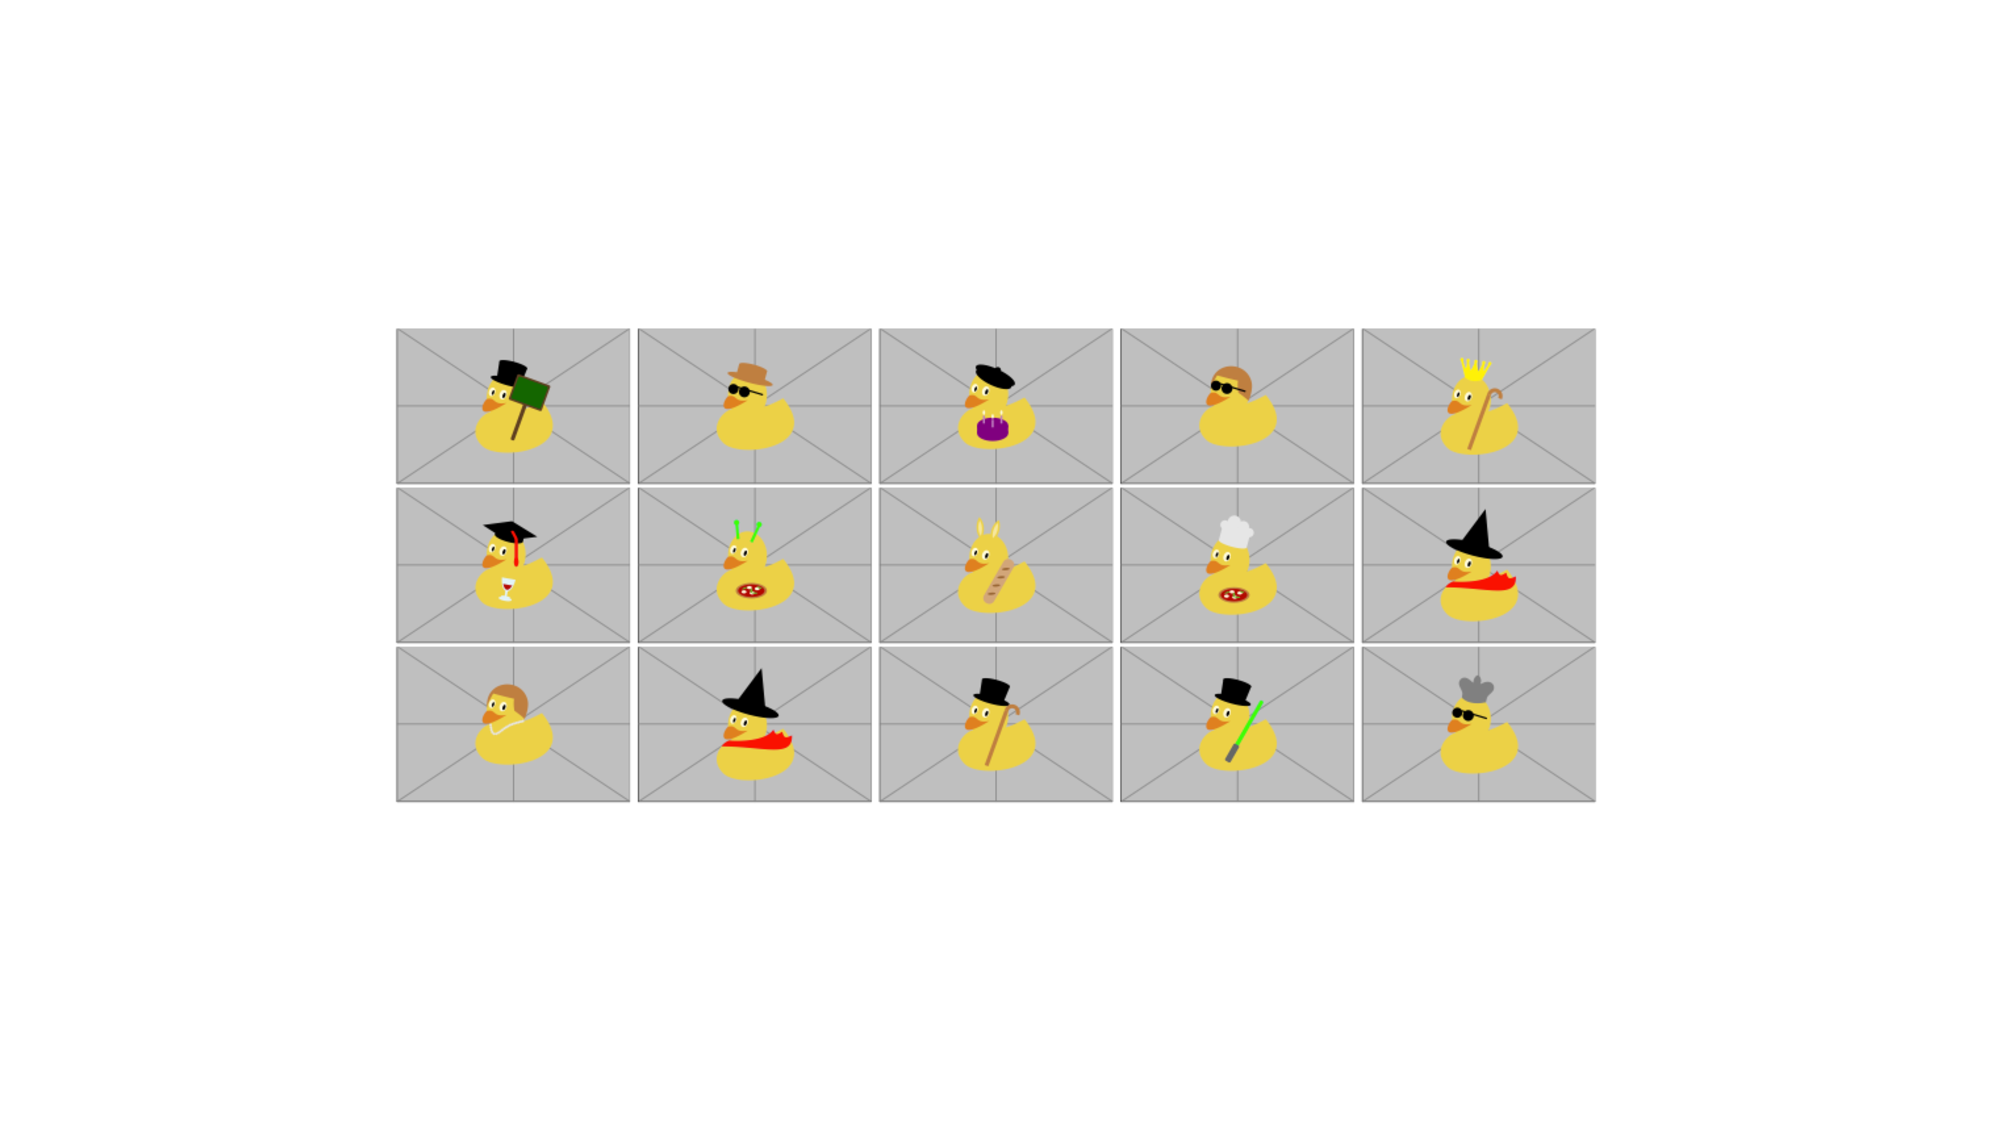
\includegraphics[width=\textwidth, trim={6cm 5cm 6cm 5cm},clip,page=1] {figures.pdf}
    \caption{Here are some photos of ducks to make you feel happy in tough times.}
    \label{fig:ducks}
\end{center}
\end{figure}


%%%%%%%%%%%%%%%%%%%%%%%%%%%%%%%%%%%%%%%%%%%%%%%%%%%%%%%%%%%%%%%%%%%%%%%%%
%% for subsections and subsubsection, I didn't particularly like having 
%% numbered environments because they appeared confusing with my objectives  
%% and task numbering. I used modified subsections and subsubsections 
%% using '\subsect' and '\subsubsect' which are unnumbered but added TOC
%%%%%%%%%%%%%%%%%%%%%%%%% RESEARCH OBJECTIVES %%%%%%%%%%%%%%%%%%%%%%%%%%%

\section{Research objectives}                   %%% suggested: 1 page limit

\subsection{Open research question}

\blindtext \cite{knuthwebsite}


\subsection{Specific research objectives}

\subsubsect{Objective 1: Some major objective here}

\blindtext

%% add more objectives 


\subsection{Tentative outline of the thesis}



%%%%%%%%%%%%%%%%%%%%%%% METHODOLOGY AND RESULTS %%%%%%%%%%%%%%%%%%%%%%%%%

\section{Proposed methodology and results}      %%% suggested: 4 page limit

%% remove the following and add your text
\blindtext


\subsection{Task 1: Major project task heading here related to objective 1}

%% remove the following and add your text
\blindtext


\subsubsect{Subtask 1.1: Some sub-task here}

%% remove the following and add your text
\blindtext


\begin{table}[ht]
\centering
\begin{tabular}{c c c c} 
\toprule \toprule
Col1 & Col2 & Col2 & Col3 \\ 
\toprule \toprule
1 & 6 & 87837 & 787 \\ 
2 & 7 & 78 & 5415 \\
3 & 545 & 778 & 7507 \\
4 & 545 & 18744 & 7560 \\
5 & 88 & 788 & 6344 \\ 
\bottomrule
\end{tabular}
\caption{Table to test captions and labels taken from Overleaf.}
\label{table:1}
\end{table}



\subsubsect{Subtask 1.2: Some other sub-task here}

%% remove the following and add your text
\blindtext


%%%% add more tasks and subtasks here


%%%%%%%%%%%%%%%%%%%%%%%%%%%%%% PUBLICATIONS %%%%%%%%%%%%%%%%%%%%%%%%%%%%

\section{Planned publications}


%% \mybibexclude makes sure these papers do not appear in the bibliographic references.
%% in case you have the same paper cited somewhere else in the text and want it  
%% to appear in the final bibliography, remove the \mybibexclude{} command 

\begin{enumerate} [leftmargin=0.6cm,itemsep=-0.5\baselineskip]
    \item \fullcite{einstein}. \mybibexclude{einstein}
    \item \fullcite{knuth-fa}. \hfill (In preparation) \mybibexclude{knuth-fa} 
\end{enumerate}



%%%%%%%%%%%%%%%%%%%%%%%%%%%%%%% TIMELINE %%%%%%%%%%%%%%%%%%%%%%%%%%%%%%

\section{Timeline}

%% this is an example of how to draw something using TikZ (REMOVE IT)
%% I used a Timeline chart made using Excel/ PowerPoint combination
\begingroup
\begin{tikzpicture}
    % draw a horizontal line   
    \draw[thick, -Triangle] (0,0) -- (\textwidth,0) node[font=\scriptsize,below left=3pt and -8pt]{years};
    
    % draw vertical lines
    \foreach \x in {0,1,...,10}
    \draw (\x cm,3pt) -- (\x cm,-3pt);
    
    \foreach \x/\descr in {4/t-2,5/t-1,6/t,7/t+1}
    \node[font=\scriptsize, text height=1.75ex,
    text depth=.5ex] at (\x,-.3) {$\descr$};
    
    % colored bar up
    \foreach \x/\perccol in
    {1/100,2/75,3/25,4/0}
    \draw[lightgray!\perccol!red, line width=4pt] 
    (\x,.5) -- +(1,0);
    \draw[-Triangle, dashed, red] (5,.5) --  +(1,0);
    
    % colored bar down
    \foreach \x/\perccol in
    {3/100,4/75,5/0}
    \draw[lightgray!\perccol!green, line width=4pt] 
    (\x,-.7) -- +(1,0);
    \draw[-Triangle, dashed, green] (6,-.7) --  +(1,0);
    
    % braces
    \draw [thick ,decorate,decoration={brace,amplitude=5pt}] (4,0.7)  -- +(2,0) 
           node [black,midway,above=4pt, font=\scriptsize] {Training period};
    \draw [thick,decorate,decoration={brace,amplitude=5pt}] (6,-.9) -- +(-1,0)
           node [black,midway,font=\scriptsize, below=4pt] {Testing period};
\end{tikzpicture}
\captionof{figure}{An abstract timeline to finish my PhD. Drawing credit goes to a user on StackExchange.}
\endgroup

%%%%%%%%%%%%%%%%%%%%%%%%%%% ACKNOWLEDGEMENT %%%%%%%%%%%%%%%%%%%%%%%%%%%%

%%%% unnumbered section but added to the TOC: `\sect`
\sect{Acknowledgement}

%% remove this and add your acknowledgement statements here
\blindtext

%%%%%%%%%%%%%%%%%%%%%%%%%%%%% BIBLIOGRAPHY %%%%%%%%%%%%%%%%%%%%%%%%%%%%%

\clearpage \phantomsection
\BibTextSpacing
\printbibliography[title={Bibliographic references},
    heading=bibintoc,notcategory=mypapers]
\clearpage
    

%%%%%%%%%%%%%%%%%%%%%%%%%%% END BIBLIOGRAPHY %%%%%%%%%%%%%%%%%%%%%%%%%%%


%%%%%%%%%%%%%%%%%%%%%%%%%%%%% END MAIN TEXT %%%%%%%%%%%%%%%%%%%%%%%%%%%%


\end{document}

%%%%%%%%%%%%%%%%%%%%%%%%%%%%% END DOCUMENT %%%%%%%%%%%%%%%%%%%%%%%%%%%%%
